\clearpage
\setcounter{figure}{0}
\setcounter{table}{0}
\renewcommand{\thefigure}{S\arabic{figure}}
\renewcommand{\thetable}{S\arabic{table}}
\section*{Supplementary material}
\addcontentsline{toc}{section}{Supplementary material}

\subsection*{S1. Verbatim source extracts for load-bearing claims}

Three claims carry the argument: the primary account of the flight, the tibia
fracture threshold behind the biomechanics, and the medieval wind regime behind the
climatology. We quote each source directly so the reader can check our reading.

\paragraph{S1.1 The flight, the distance, the injury, and the tail.}
The entire factual basis is one passage of William of Malmesbury, \textit{Gesta
Regum Anglorum} (book II, ch. 225), in the Oxford Medieval Texts edition
\autocite{williamMalmesbury_gesta}. The Latin reads:

\begin{quote}\small\itshape
Is erat litteris, quantum ad id temporis, bene imbutus, aeuo maturus, immanem
audaciam prima iuuentute conatus: nam pennas manibus et pedibus haud scio qua
innexuerat arte, ut Daedali more uolaret, fabulam pro uero amplexus, collectaque e
summo turris aura, spatio stadii et plus uolauit; sed uenti et turbinis uiolentia,
simul et temerarii facti conscientia, tremulus cecidit, perpetuo post haec debilis,
et crura effractus. Ipse ferebat causam ruinae quod caudam in posteriori parte
oblitus fuerit.
\end{quote}

\noindent In the standard English rendering:

\begin{quote}\small
He had by some means, I scarcely know what, fastened wings to his hands and feet so
that, mistaking fable for truth, he might fly like Daedalus, and, collecting the
breeze on the summit of a tower, he flew for more than the distance of a furlong.
But, agitated by the violence of the wind and the swirling of air, as well as by
awareness of his rashness, he fell, broke his legs, and was lame ever after. He
himself used to say that the cause of his failure was his forgetting to put a tail
on the back part.
\end{quote}

\noindent Every element we model is in these two sentences: the tower launch, the
hand-and-foot wings, the breeze, the furlong (a stadium, about \SI{200}{\meter}),
the loss of control in gusty air, the broken legs and permanent lameness, and the
diagnosis (\textit{caudam \ldots oblitus}, ``forgetting a tail'').

\paragraph{S1.2 The tibia fracture threshold.}
The \SIrange{7.5}{11.3}{\kilo\newton} per-leg band in \cref{fig:biomech} comes from
the injury-biomechanics literature, consolidated in a recent systematic review
\autocite{abidin2026tibia}, which reports that

\begin{quote}\small
tibial fracture thresholds range from \(\sim\)7.5 kN in female specimens to 11.3 kN
under combined axial and bending loads, with fibula contribution increasing axial
tolerance by \(\sim\)10\%.
\end{quote}

\noindent The upper figure traces to the primary compilation of
\textcite{salzar2014leg}, which recommends a tibial axial threshold of
\(\sim\)\SI{10.3}{\kilo\newton} rising to \(\sim\)\SI{11.3}{\kilo\newton} with the
fibula's contribution. We use the range, not a point value, precisely because the
threshold depends on sex, loading rate, and bending.

\paragraph{S1.3 The medieval wind regime.}
The claim that modern reanalysis is a reasonable, probably conservative proxy for
Eilmer's epoch rests on reconstructions of the North Atlantic Oscillation, which
disagree on timing. \textcite{trouet2009nao} report

\begin{quote}\small
a 947-year-long multidecadal North Atlantic Oscillation (NAO) reconstruction [with]
a persistent positive NAO during the MCA [Medieval Climate Anomaly].
\end{quote}

\noindent The later, model-tested reconstruction of \textcite{ortega2015nao}
revises this, finding

\begin{quote}\small
no persistent positive NAO during the medieval period, but [suggesting] that
positive phases were dominant during the thirteenth and fourteenth centuries.
\end{quote}

\noindent We therefore make only the weaker claim the evidence supports: neither
reconstruction indicates the weak westerlies of a negative NAO over Britain in
Eilmer's period, so the favourable-wind fraction we compute from 2004--2023 ERA5
(\cref{fig:wind}) is not an overestimate for the eleventh century. We do not rely on
medieval winds being \emph{stronger} than modern ones.

\subsection*{S2. Monte Carlo parameter priors}

\Cref{tab:priors} lists the plausible ranges sampled in the feasibility envelope
(\cref{fig:montecarlo}). All priors are uniform over the stated range.

\begin{table}[htbp]
  \centering
  \caption{\textbf{Sampled parameter ranges for the Monte Carlo
  (\cref{fig:montecarlo}).} Launch wind is not sampled from a prior but drawn from
  the empirical ERA5 SW-sector launchable speeds (\cref{fig:wind}).}
  \label{tab:priors}
  \small
  \begin{tabular}{lll}
    \toprule
    Parameter & Range & Basis \\
    \midrule
    Wing area & \SIrange{5}{10}{\meter\squared} & crude hand/foot wing \\
    All-up mass & \SIrange{70}{90}{\kilogram} & adult pilot plus apparatus \\
    Trim \(C_L\) & \numrange{0.7}{1.1} & cambered cloth, low Reynolds number \\
    Glide ratio \LD & \numrange{3}{7} & hang-glider class, crude build \\
    Tower height & \SIrange{15}{25}{\meter} & abbey tower, conservative \\
    Escarpment slope & \ang{8}--\ang{18} & DEM p90 as a floor \\
    Ridge-lift efficiency & \numrange{0.5}{1.0} & attached-upslope fraction \\
    Centre of gravity & \numrange{0.35}{0.55}\,\(c\) & hanging-pilot range \\
    Aspect ratio & \numrange{3}{5} & span/area of a hand-foot wing \\
    Tail neutral-point shift & \numrange{0.18}{0.32}\,\(c\) & tail size variation \\
    \bottomrule
  \end{tabular}
\end{table}

\subsection*{S3. Ridge-lift field}

\Cref{fig:ridge} shows the first-order orographic lift field summarised in the main
text. We keep the full field here because the smoothed \SI{6}{\meter} DEM makes the
modelled slope, and therefore the lift, a lower bound; the main analysis carries
only its magnitude.

\begin{figure}[htbp]
  \centering
  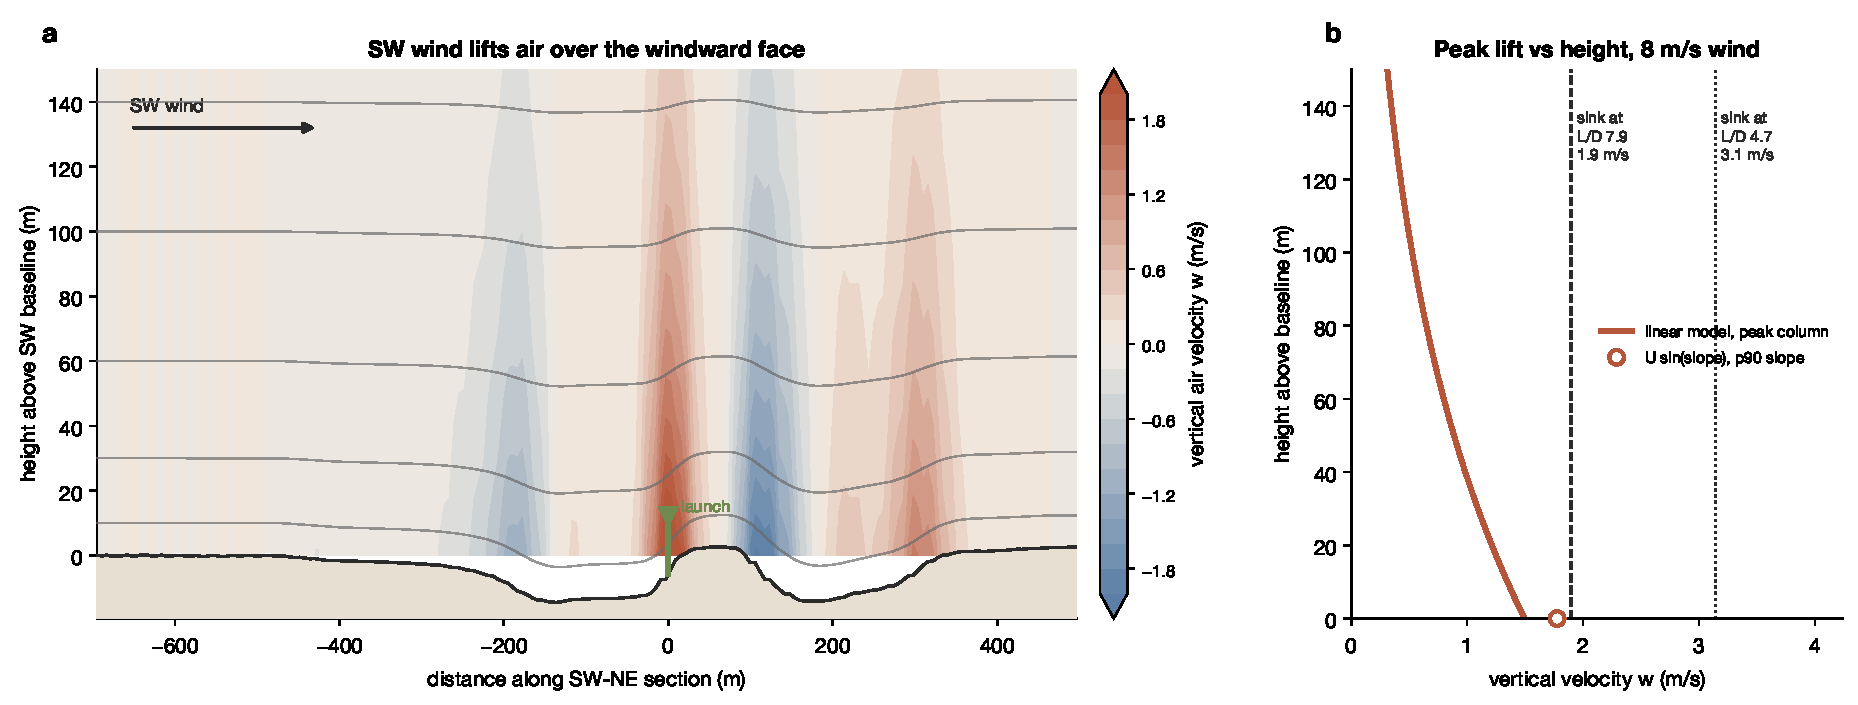
\includegraphics[width=\linewidth]{fig3_ridge_lift}
  \caption{\textbf{Ridge lift over the escarpment matches a crude glider's sink.}
  A first-order linear orographic model (\(w = U\,\mathrm{d}h/\mathrm{d}x\,e^{-kz}\))
  over the real SW--NE terrain section.
  \textbf{(a)} Vertical-velocity field and streamlines for an
  \SI{8}{\meter\per\second} southwest wind.
  \textbf{(b)} Lift versus height above the windward face. Peak lift just southwest
  of the abbey is about \SI{1.5}{\meter\per\second}, above a crude glider's
  optimistic sink of \SIrange{0.75}{1.0}{\meter\per\second}, with a soarable band
  about \SI{38}{\meter} deep.}
  \label{fig:ridge}
\end{figure}
